\subsection{Analysis and Limitations}
\label{subsec:analysis_limitations}

\subsubsection{Comparison with the Closest Prior Work}
\label{subsec:vs_mambaofr}

MgfrOFR is built directly on top of MambaOFR~\cite{mao2025mambaofr}, so the contribution must be separated from the baseline backbone. We do not claim originality for bidirectional Mamba propagation, the degradation-aware prompt block, or the original reconstruction head. The contribution of this work lies in how propagated features are reorganized and regularized before reconstruction.

Compared with MambaOFR, MgfrOFR differs in four aspects. First, the propagated feature is no longer treated as a single restoration carrier; MGFE exposes explicit coarse-to-fine branches. Second, these branches are summarized and fed back through channel-wise recalibration rather than being used only for auxiliary supervision. Third, branch diversity is constrained by ranking correlation on temporal correspondences, rather than by an identity-based objective inherited from recognition tasks. Fourth, RATR is used only during training, so the deployment interface remains compatible with the baseline inference pipeline.

The key value of this design is representation-level symmetry. MgfrOFR does not treat object-level geometric regularity as the target; instead, it studies how an AI restoration model can maintain balanced coarse-to-fine feature spaces under asymmetric film degradation. MGFE separates evidence by restoration granularity, while RATR keeps temporal-similarity rankings from becoming redundant across branches. This provides a concrete symmetry-related mechanism without overstating the mathematical scope of the method.

\subsubsection{MGFE--RATR Synergy for Branch Balance}
\label{subsec:synergy}

The ablation study indicates that MGFE and RATR have different roles in the full model. RATR acts as a diversity regularizer that makes branches more complementary, while MGFE recalibration alone mainly improves fidelity (Table~\ref{tab:ablation}). In the RATR-only configuration, MGFE branch descriptors are still computed and used as multi-granularity ranking targets; only the channel-wise scale/shift feedback is disabled. MGFE therefore creates the branch structure needed for coarse-to-fine feature balance, whereas RATR suppresses redundant temporal-ranking behavior.

The asymmetric ablation behavior in Table~\ref{tab:ablation} shows that MGFE recalibration alone improves the baseline but does not reach the fidelity--perception balance of the full model. This is consistent with the perception--distortion trade-off~\cite{blau2018perception}, which establishes that optimizing a distortion measure such as PSNR does not by itself guarantee the best perceptual behavior. The channel-wise recalibration in Equation~\eqref{eq:recalibration} is conditioned on an averaged branch context and is driven mainly by the pixel reconstruction loss. Without a diversity constraint, the granularity branches can converge toward similar low-frequency corrections, so the MGFE-only variant remains less effective than the full model on LPIPS and DISTS. RATR mitigates this effect by acting on branch-ranking structure rather than on pixel error. Penalizing correlated temporal rankings across branches (Equations~\eqref{eq:loss_intra}--\eqref{eq:loss_ratr}) prevents the branches from collapsing onto a single fidelity-oriented direction and preserves complementary fine-grained evidence. The full model therefore gives the strongest combined fidelity and perceptual result.

The real-world results are consistent with this interpretation but do not prove content fidelity without ground truth. On the SRWOV real-world test set (Table~\ref{tab:realworld}), MgfrOFR achieves the best NIQE (5.12) and improves BRISQUE relative to MambaOFR (24.79 vs.\ 29.79), while RTN keeps the best BRISQUE score and MgfrOFR's CLIP-IQA+ (0.4092) is lower than OldPhoto, MambaOFR, and RTN. This pattern suggests that the multi-granularity decomposition transfers useful restoration structure beyond the synthetic training distribution, but the no-reference gains should be interpreted as evidence of statistical naturalness rather than definitive perceptual superiority.

\subsubsection{Branch Balance Analysis}
\label{subsec:branch_analysis}

To verify that the three granularity branches capture complementary restoration cues rather than correlated copies of the same evidence, we analyze the pairwise cosine similarity between branch descriptors across the SRWOV synthetic test set. This analysis directly tests the feature-space symmetry claim: balanced branches should remain comparable but not redundant.

The full model yields lower inter-branch similarity than the MGFE-only variant (Figures~\ref{fig:branch_similarity} and~\ref{fig:branch_error_map}), confirming that RATR is not just an auxiliary loss but the mechanism that keeps the granularity branches functionally distinct. The RATR-only variant remains closer to the full model than to MGFE-only, showing that ranking diversity regularization already suppresses collapse even before the recalibration feedback is enabled.

Figure~\ref{fig:branch_similarity} illustrates this contrast for a representative frame. In the MGFE-only configuration, the off-diagonal similarities remain high, indicating that the branches still encode nearly the same restoration evidence. In the full model, these off-diagonal values drop markedly, especially for the fine-grained branch, demonstrating that RATR produces a more differentiated and balanced branch geometry.

\begin{figure}[!t]
\centering
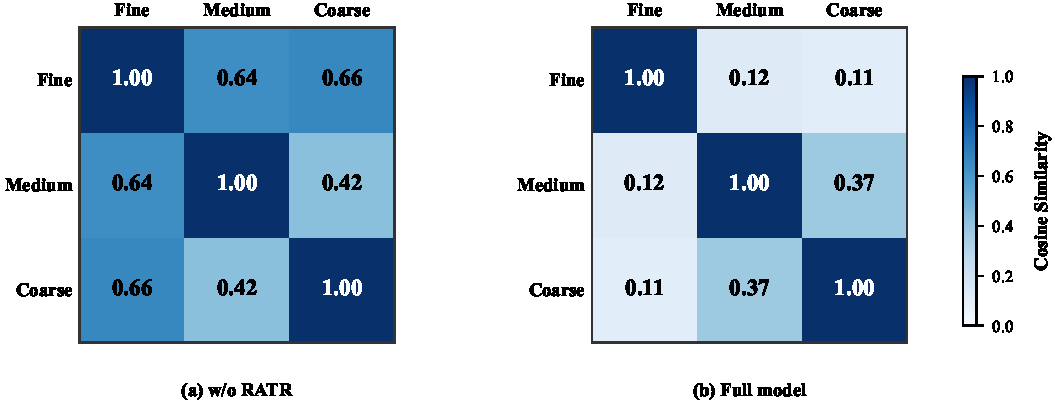
\includegraphics[width=0.84\textwidth]{figures/Fig9a_branch_similarity.pdf}
\caption{Branch balance analysis. Pairwise cosine similarity is compared between the MGFE-only configuration and the full MgfrOFR model under the 30-clip REDS synthetic protocol. RATR reduces off-diagonal similarity from 0.85--0.90 to 0.23--0.31, confirming that ranking-aware regularization prevents granularity branches from collapsing into correlated descriptors.\label{fig:branch_similarity}}
\end{figure}

\begin{figure}[!t]
\centering
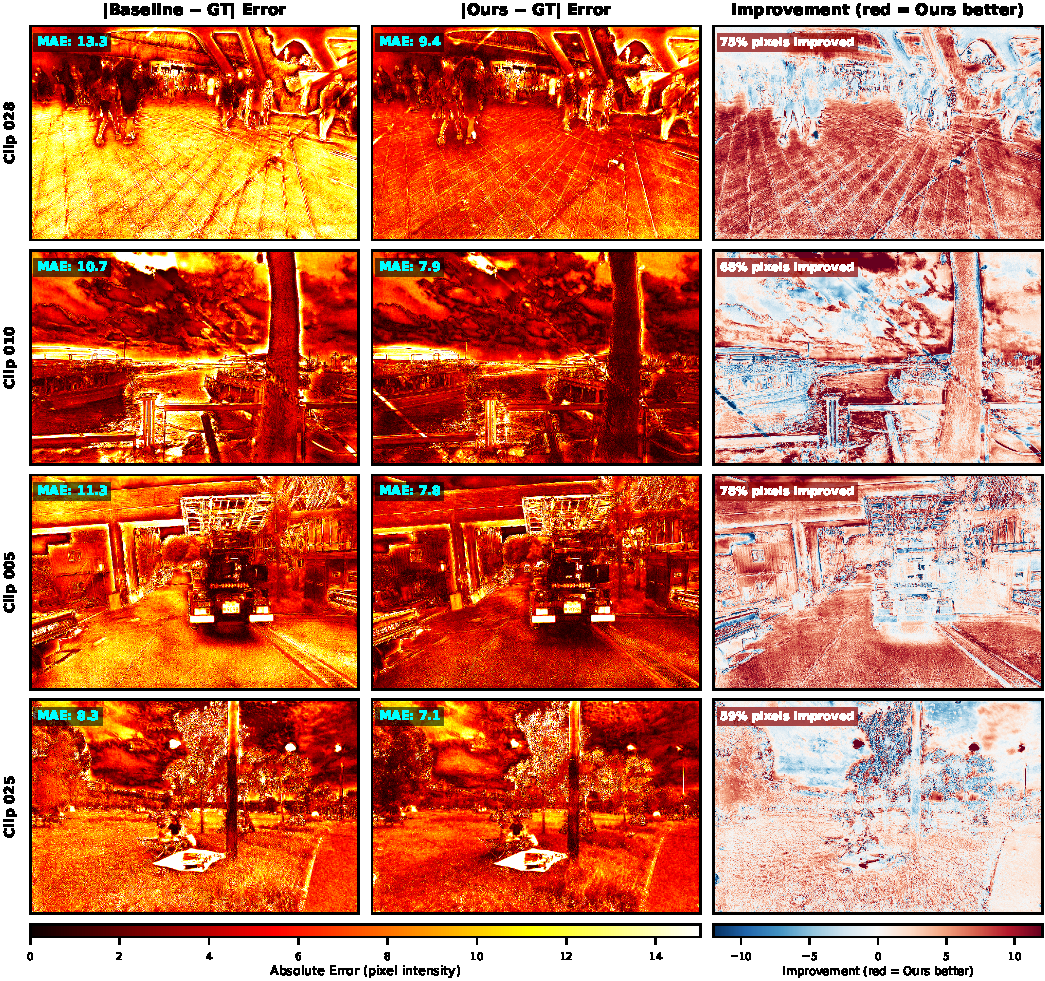
\includegraphics[width=0.98\textwidth]{figures/Fig9b_error_map.pdf}
\caption{Pixel-wise absolute-error comparison on four representative synthetic frames. The left and middle columns compare $|$MambaOFR $-$ GT$|$ and $|$MgfrOFR $-$ GT$|$; the right column illustrates their difference, where red indicates regions in which MgfrOFR reduces the reconstruction error. The error maps demonstrate that lower branch correlation translates into spatially broader restoration gains rather than isolated local fixes.\label{fig:branch_error_map}}
\end{figure}

Building on the similarity analysis, we qualitatively observe a consistent specialization pattern. The fine-grained branch is most sensitive to localized defects such as scratches and pixel-level noise; the coarse branch emphasizes broader structural corruption such as blotches and cracks; and the medium branch occupies an intermediate role. This behavior is consistent with progressive token fusion, where fewer surviving tokens aggregate over wider spatial support. The pixel-domain error maps in Figure~\ref{fig:branch_error_map} further demonstrate that this branch decorrelation translates into spatially broader restoration gains rather than isolated local fixes.

\subsubsection{When Does MgfrOFR Struggle?}
\label{subsec:failure}

MgfrOFR's advantage is not uniform across all degradation conditions. The ablation and sensitivity results indicate that the full model is most useful when heterogeneous degradation is present, such as structural damage co-occurring with fine scratches in the same frame. On clips dominated by a single degradation type, such as uniform flicker without spatial damage, the multi-granularity decomposition can add representational overhead without proportional benefit, and the baseline or RATR-only variant may match the full model's fidelity.

The real-world CLIP-IQA+ result highlights a trade-off between naturalness and enhancement-oriented perceptual quality. MgfrOFR's CLIP-IQA+ (0.4092) is below OldPhoto (0.4503), MambaOFR (0.4351), and RTN (0.4163), while MgfrOFR achieves the best NIQE (5.12) and improves BRISQUE relative to MambaOFR (24.79 vs.\ 29.79). This pattern reflects that different no-reference metrics measure distinct aspects of restoration quality. CLIP-IQA+ is trained on human quality annotations that correlate with sharp textures and high-contrast details~\cite{wang2023clipiqa}, favoring methods that enhance perceptual sharpness through learned global priors. NIQE and BRISQUE instead measure statistical deviation from natural image distributions and penalize artifacts introduced by texture hallucination. MgfrOFR's granularity-based recalibration operates conservatively on the propagated feature stream, which appears to preserve statistical naturalness while providing less texture enhancement than the stronger CLIP-IQA+ baselines. For archival restoration, NIQE/BRISQUE may be more relevant proxies when content fidelity is prioritized, but a human study is needed to validate that preference.

\subsubsection{Limitations, Threats to Validity, and Future Work}
\label{subsec:limitations}

\paragraph{Threats to Validity.}
Five threats affect the interpretation of the results. \textbf{Dataset threat}: all training uses synthetic degradation applied to REDS clips, which introduces a synthetic-to-real domain gap and may limit generalization to archival footage with correlated degradation chains not modeled by the pipeline. \textbf{Metric threat}: evaluation relies on PSNR/SSIM/LPIPS/DISTS for synthetic full-reference assessment and no-reference metrics for real-world assessment; these metrics emphasize different aspects of quality and may not fully align with human perceptual judgments. \textbf{Human-evaluation threat}: the study does not include an expert reader study with film-restoration practitioners or archivists, so the practical value of improvements on authentic footage is inferred from proxy metrics and qualitative inspection. \textbf{Baseline threat}: three baselines (VRT, RVRT, ShiftNet) required adaptation from video restoration to degradation specific to old film restoration, which preserves their architectures but may not reflect their optimal performance under a different training regime. \textbf{Synthetic-to-real threat}: the real-world evaluation lacks ground truth, so improvements in NIQE/BRISQUE reflect statistical naturalness rather than verified content fidelity, and the absence of external validation on additional datasets weakens the generalization claim.

\paragraph{Limitations and Future Work.}
RATR adds a training-time cost because it requires branch-wise similarity matrices over the batch-time descriptor set $\bar{N}=BT$. Its dominant cost therefore grows approximately quadratically in $\bar{N}$. Longer clips or larger effective batch-time products would make this quadratic term more pronounced, so gradient checkpointing or selective ranking construction, such as sampling a subset of anchors per iteration, will be needed for larger training settings. The second limitation is the synthetic-to-real domain gap caused by REDS-based training degradation. Although the real-world NIQE/BRISQUE results are encouraging, authentic archival footage can contain correlated degradation chains that synthetic pipelines do not model. The third limitation is evaluation scope: validation is limited to SRWOV, and additional archival datasets plus human evaluation would strengthen the generalization claim.

Promising extensions include adaptive branch activation conditioned on degradation severity, frequency-aware branch specialization that assigns structural recovery and texture restoration to dedicated branches, and joint old film restoration and colorization frameworks for archival digitization and cultural heritage restoration workflows~\cite{kokaram2004missing}.
